\begin{frame}
    \frametitle{System Model}
    \begin{figure}[H]
        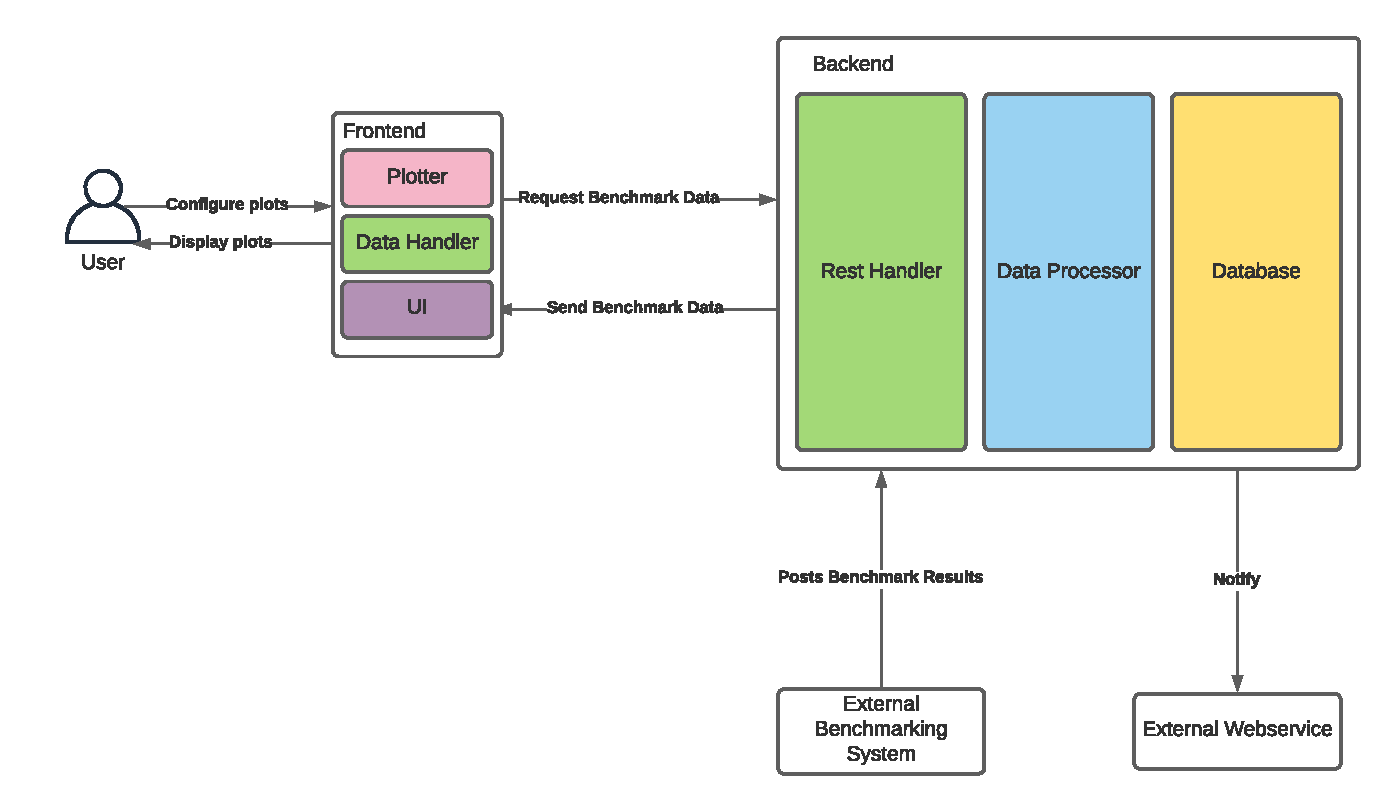
\includegraphics[width=\textwidth]{images/systemmodel.pdf}
        \label{fig:systemmodel}
    \end{figure}
\end{frame}


\begin{frame}
    \begin{columns}[T]
        \begin{column}{.48\textwidth}
            \begin{figure}[H]
                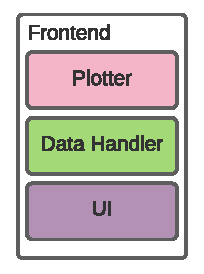
\includegraphics[width=\textwidth]{images/systemmodel_frontend.pdf}
                \label{fig:frontendmodel}
            \end{figure}
        \end{column}
        \hfill
        \begin{column}{.48\textwidth}
            \begin{block}{Frontend}
                Allows the user to interact with the application.
            \end{block}
            \begin{itemize}
                \item<2-> UI:\newline{} Handles interactions with the user.
                \item<3-> Plotter:\newline{} Generates plots.
                \item<4-> Data Handler:\newline{} Requests information from the Backend with their REST API.
            \end{itemize}
        \end{column}
    \end{columns}
\end{frame}


\begin{frame}
    \begin{columns}[T]
        \begin{column}{.48\textwidth}
            \begin{figure}[H]
                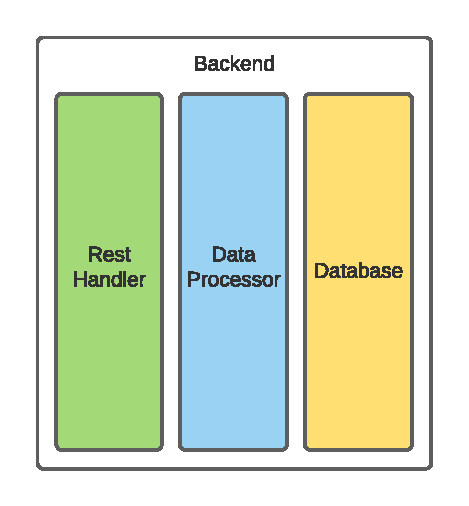
\includegraphics[width=\textwidth]{images/systemmodel_backend.pdf}
                \label{fig:backendmodel}
            \end{figure}
        \end{column}
        \hfill
        \begin{column}{.48\textwidth}
            \begin{block}{Backend}
                Handles data processing, storage, and an API to interact with.
            \end{block}
            \begin{itemize}
                \item<2-> REST Handler:\newline{} Provides the REST API, which is used by the frontend and other external web services.
                \item<3-> Data Processor:\newline{} Transforms the data for storage and computes other metrics.
                \item<4-> Storage:\newline{} Provides persistent storage for Benchmark Data.
            \end{itemize}
        \end{column}
    \end{columns}
\end{frame}


\begin{frame}
    \begin{figure}[H]
        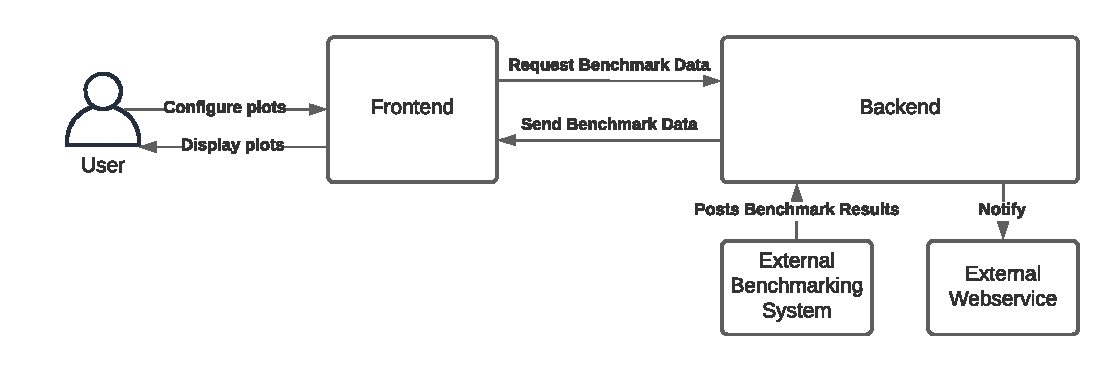
\includegraphics[width=\textwidth]{images/systemmodel_light_overview.pdf}
        \label{fig:lightoverview}
    \end{figure}

    \begin{block}{User}
        Configures Plots and Receives them.
    \end{block}
\end{frame}


\begin{frame}
    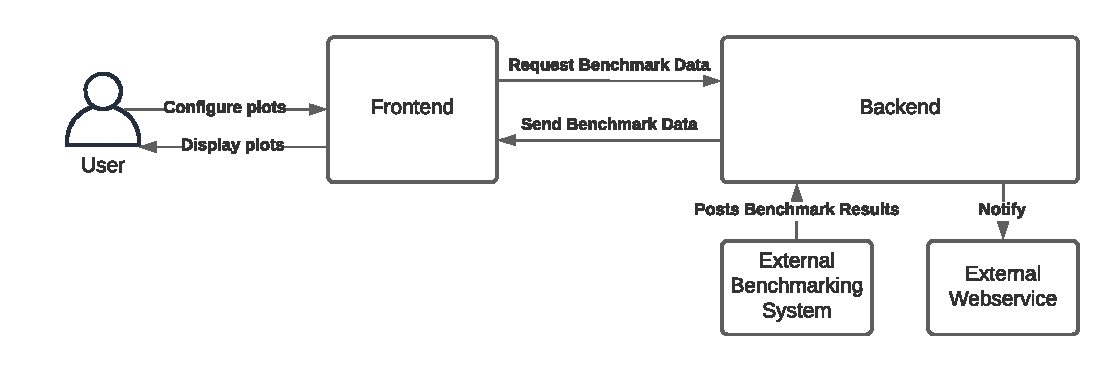
\includegraphics[width=\textwidth]{images/systemmodel_light_overview.pdf}

    \begin{block}{External Benchmarking System}
        Posts Benchmark Results to our API.
    \end{block}
\end{frame}


\begin{frame}
    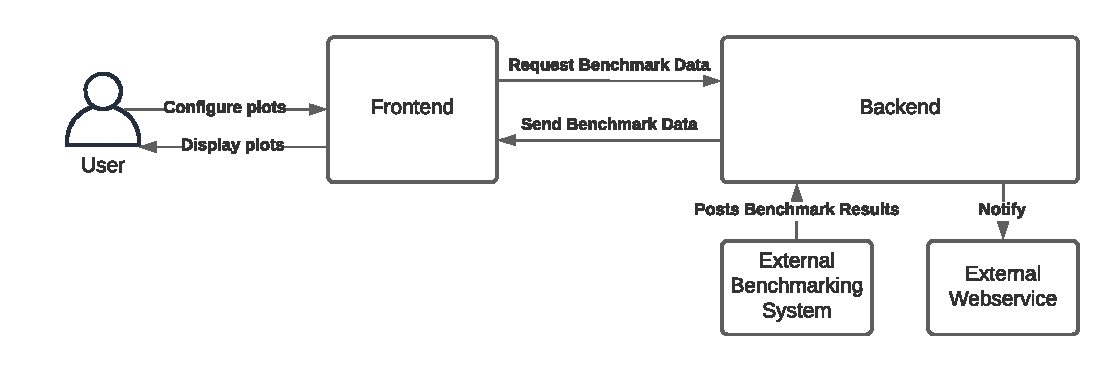
\includegraphics[width=\textwidth]{images/systemmodel_light_overview.pdf}

    \begin{block}{External Webservice}
        Gets notified, e.g. by webhook subscriptions.
    \end{block}
\end{frame}